%------------------------------------------------------------------------
% add novatel library documentation as appendix
%------------------------------------------------------------------------
\setcounter{page}{1}
\chapter{NovatelOEM4 GPS library Documentation}
\cleardoublepage
\pagestyle{empty}
\newlength{\originalVOffset}
\newlength{\originalHOffset}
\setlength{\originalVOffset}{\voffset}   
\setlength{\originalHOffset}{\hoffset}

\setlength{\voffset}{0cm}
\setlength{\hoffset}{0cm}
\label{appendix:novatel}

\includepdf[pages=5-16]{appendix/novatel-oem4-python}
\cleardoublepage


%------------------------------------------------------------------------
% add maxon library documentation as appendix
%------------------------------------------------------------------------
\setcounter{page}{1}
\setlength{\voffset}{\originalVOffset}
\setlength{\hoffset}{\originalHOffset}
\chapter{Maxon EPOS CANopen Library Documentation}
\cleardoublepage
\setlength{\voffset}{0cm}
\setlength{\hoffset}{0cm}
\label{appendix:maxon}

\includepdf[pages=5-18]{appendix/maxon-epos-canopen}
\setlength{\voffset}{\originalVOffset}
\setlength{\hoffset}{\originalHOffset}
\cleardoublepage

%------------------------------------------------------------------------
% add 3D printed drawings as appendix
%------------------------------------------------------------------------
\setcounter{page}{1}
\pagestyle{plain}
\setlength{\voffset}{\originalVOffset}
\setlength{\hoffset}{\originalHOffset}
\chapter{Sensor support Drawings}
\label{appendix:sensor_drawings}
\pagebreak

%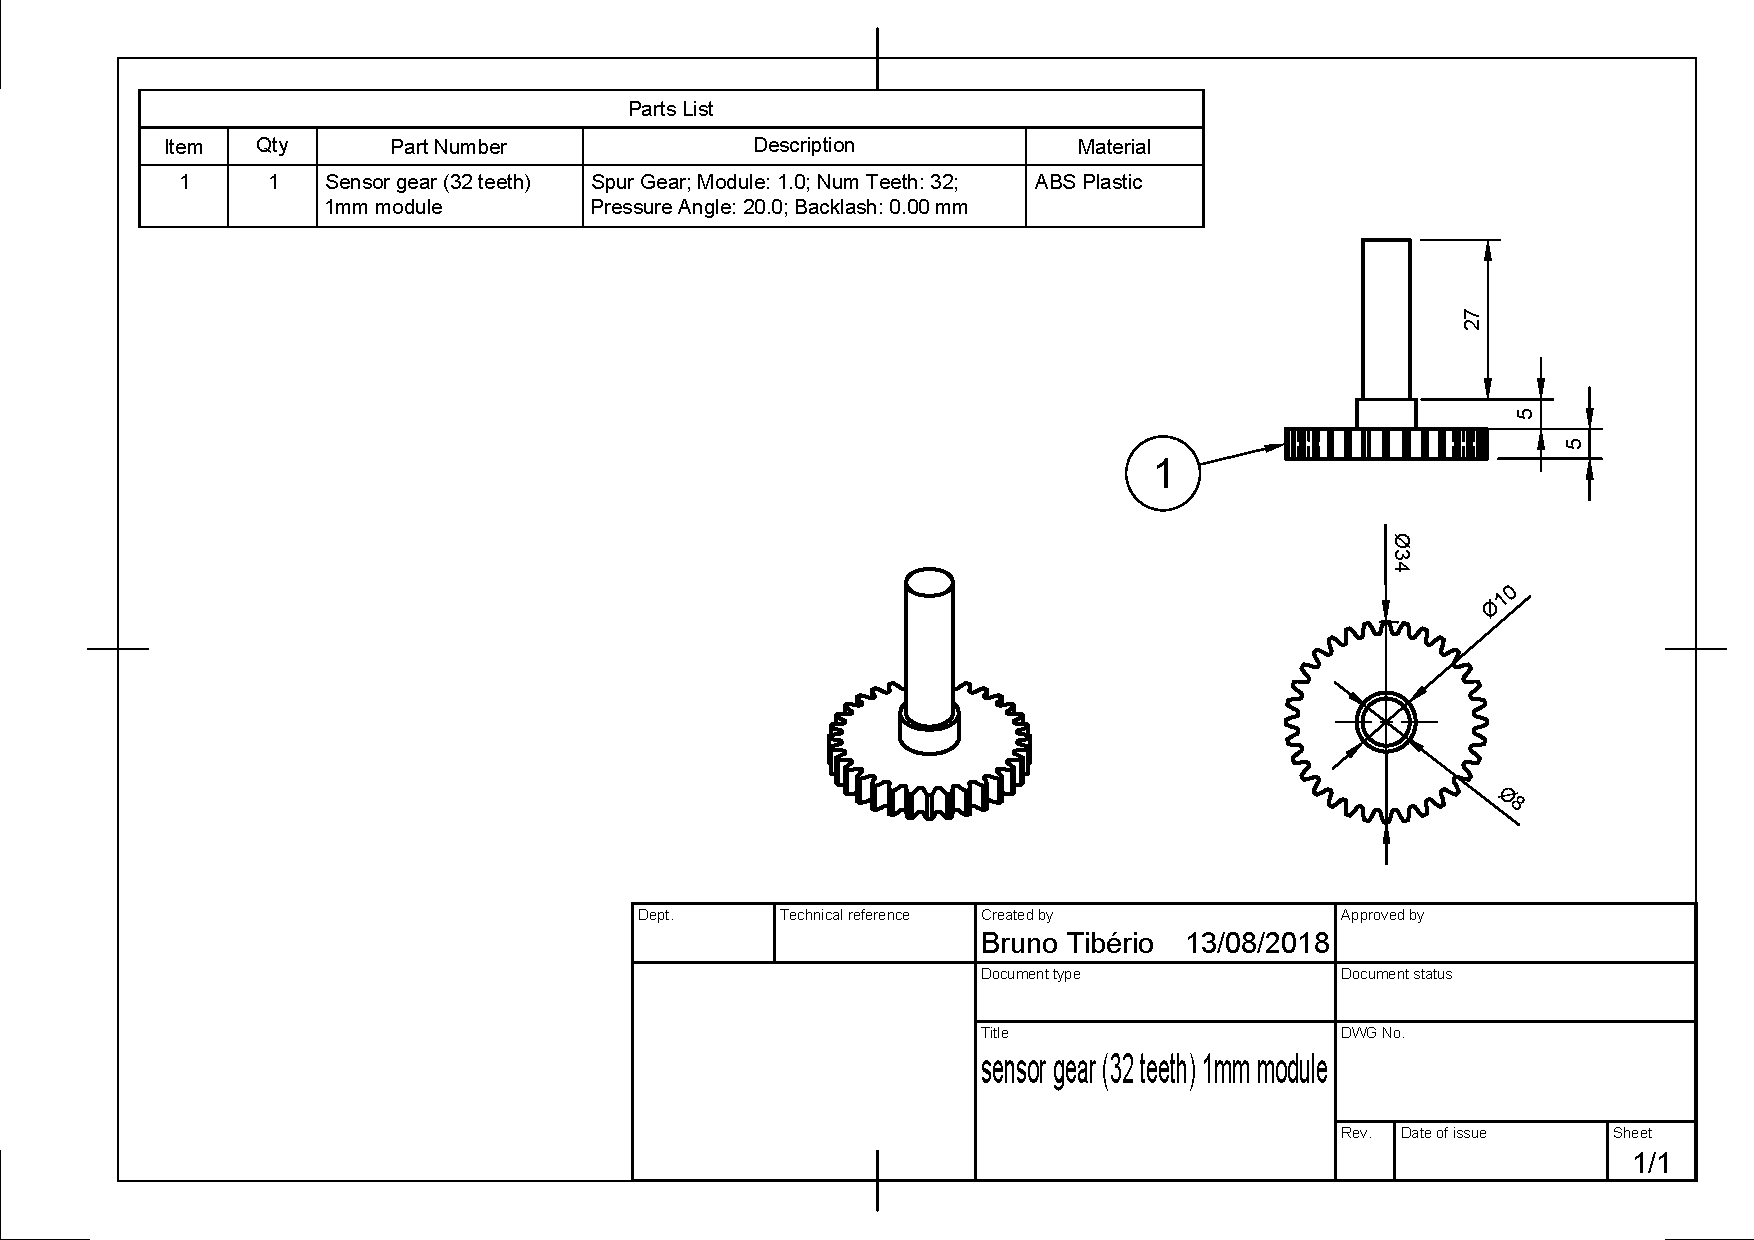
\includepdf[scale=0.75, angle=-90, pagecommand=\section{Sensor gear 32 teeth} \label{draw:sensor-gear}, offset=0 -0.5cm, trim=5mm 5mm 5mm 5mm,clip]{Drawings/sensor-gear}
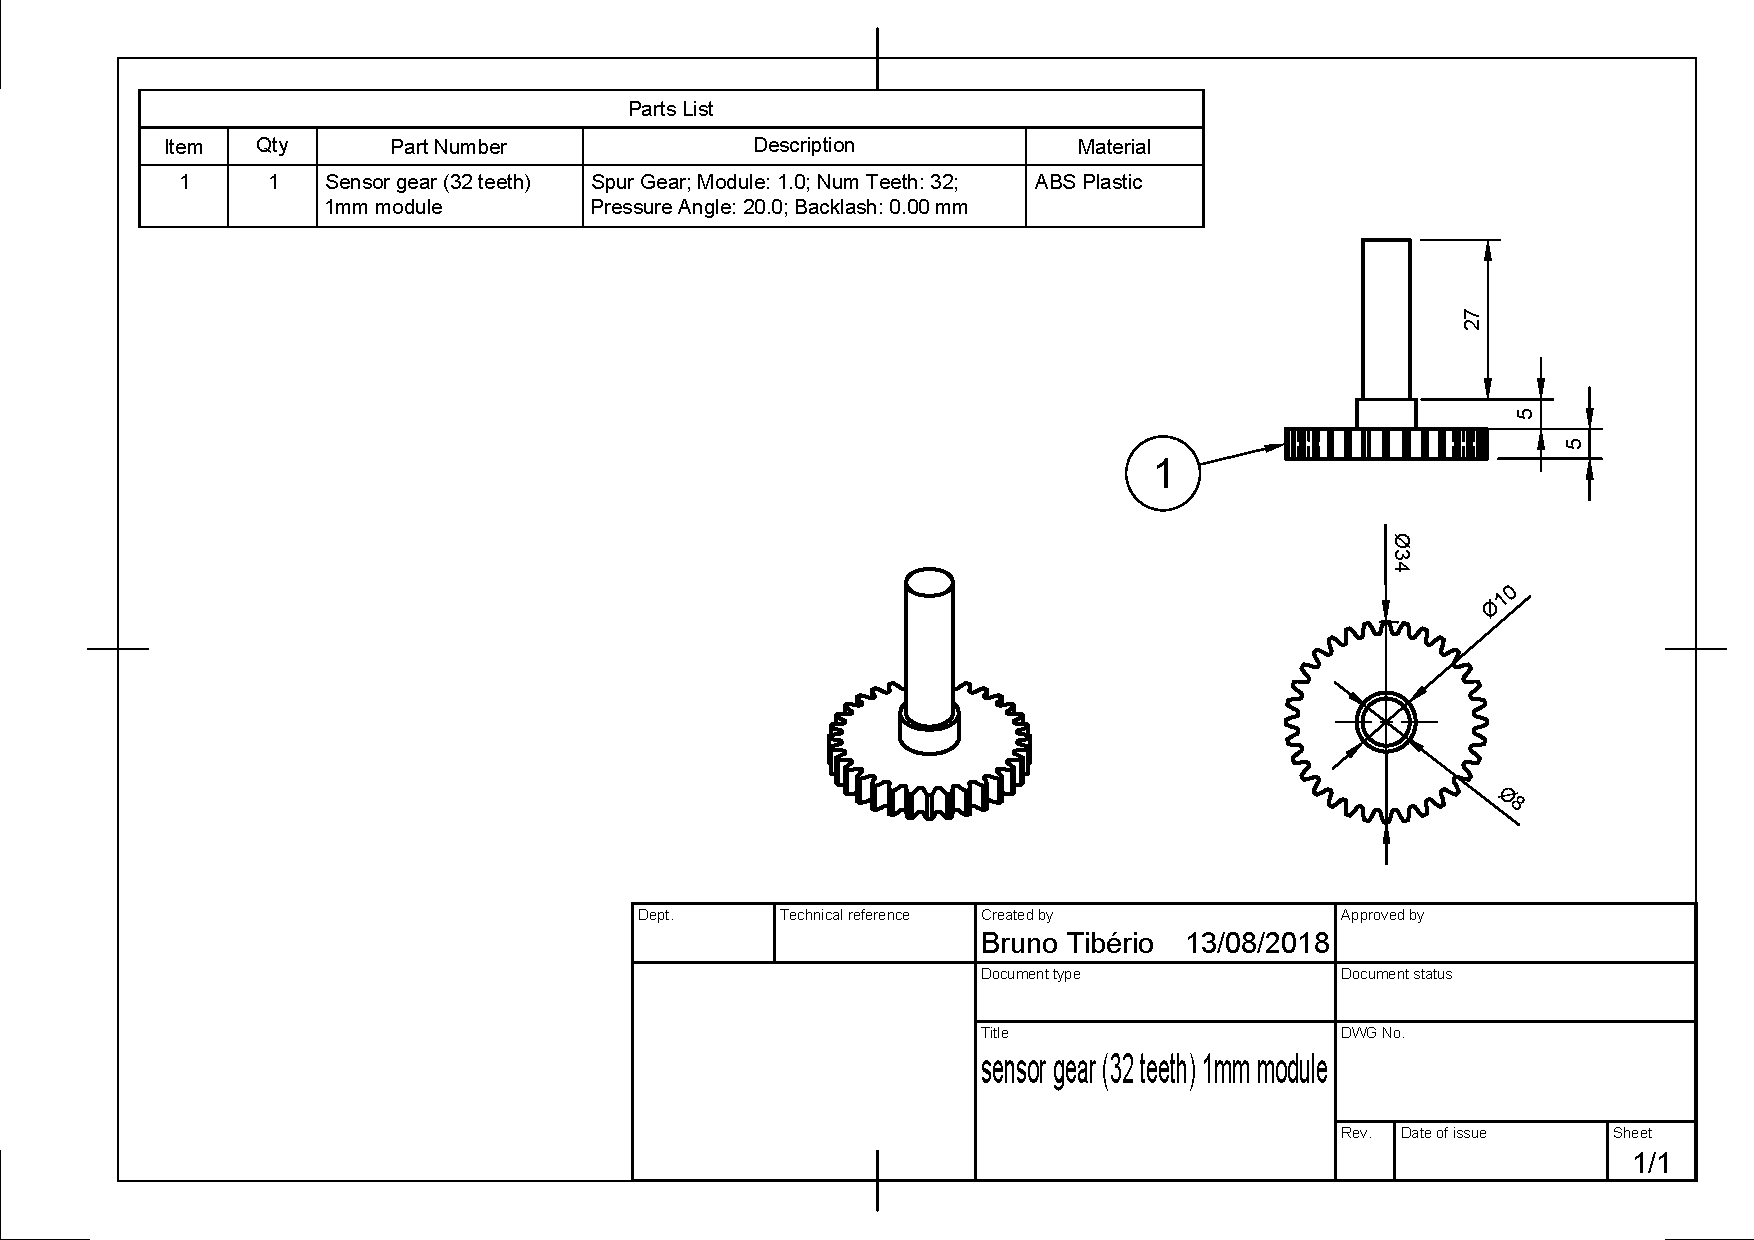
\includepdf[scale=0.8, landscape=true, pagecommand=\section{Sensor gear 32 teeth} \label{draw:sensor-gear}, trim=5mm 5mm 5mm 5mm,clip]{Drawings/sensor-gear}

%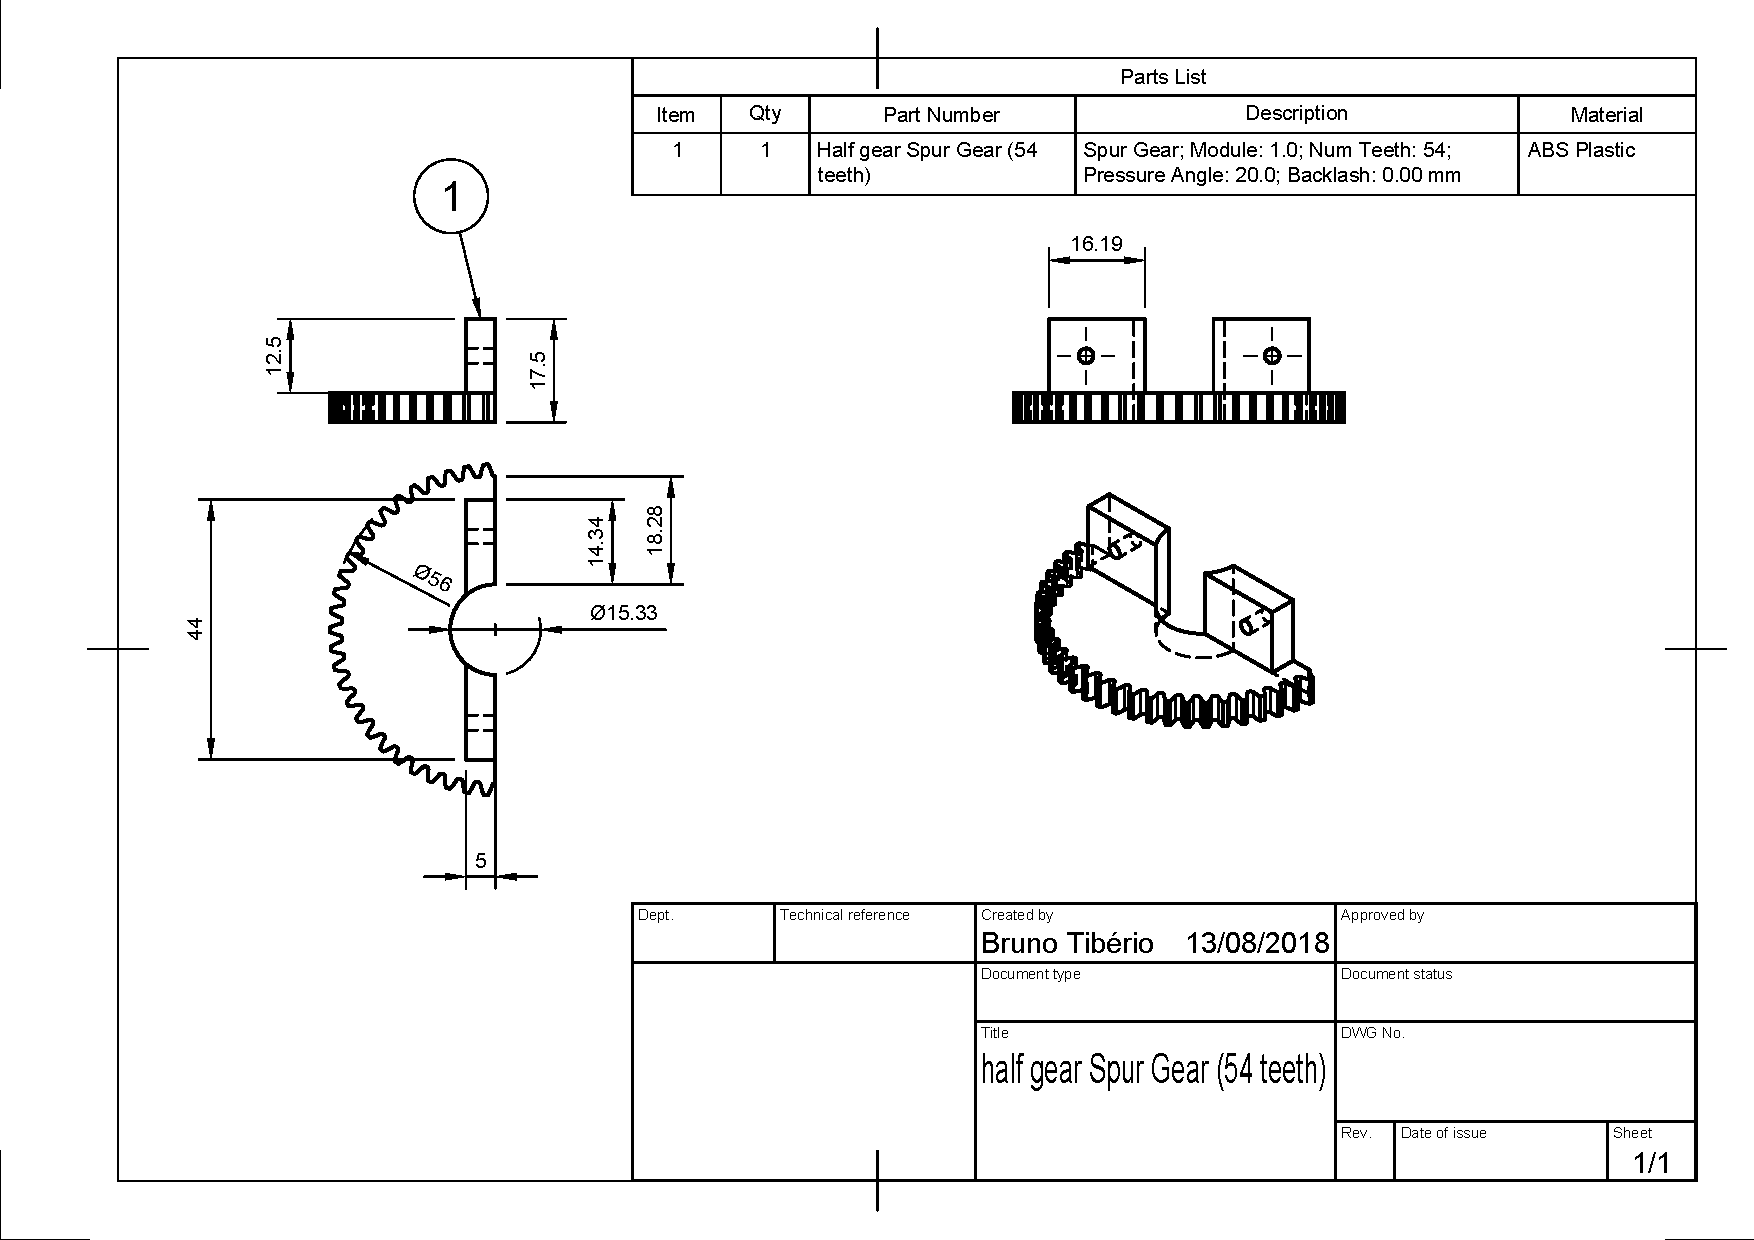
\includepdf[scale=0.75, angle=-90,pagecommand=\section{Half gear 54 teeth} \label{draw:half-gear}, offset=0 -0.5cm, trim=5mm 5mm 5mm 5mm,clip]{Drawings/half-gear}
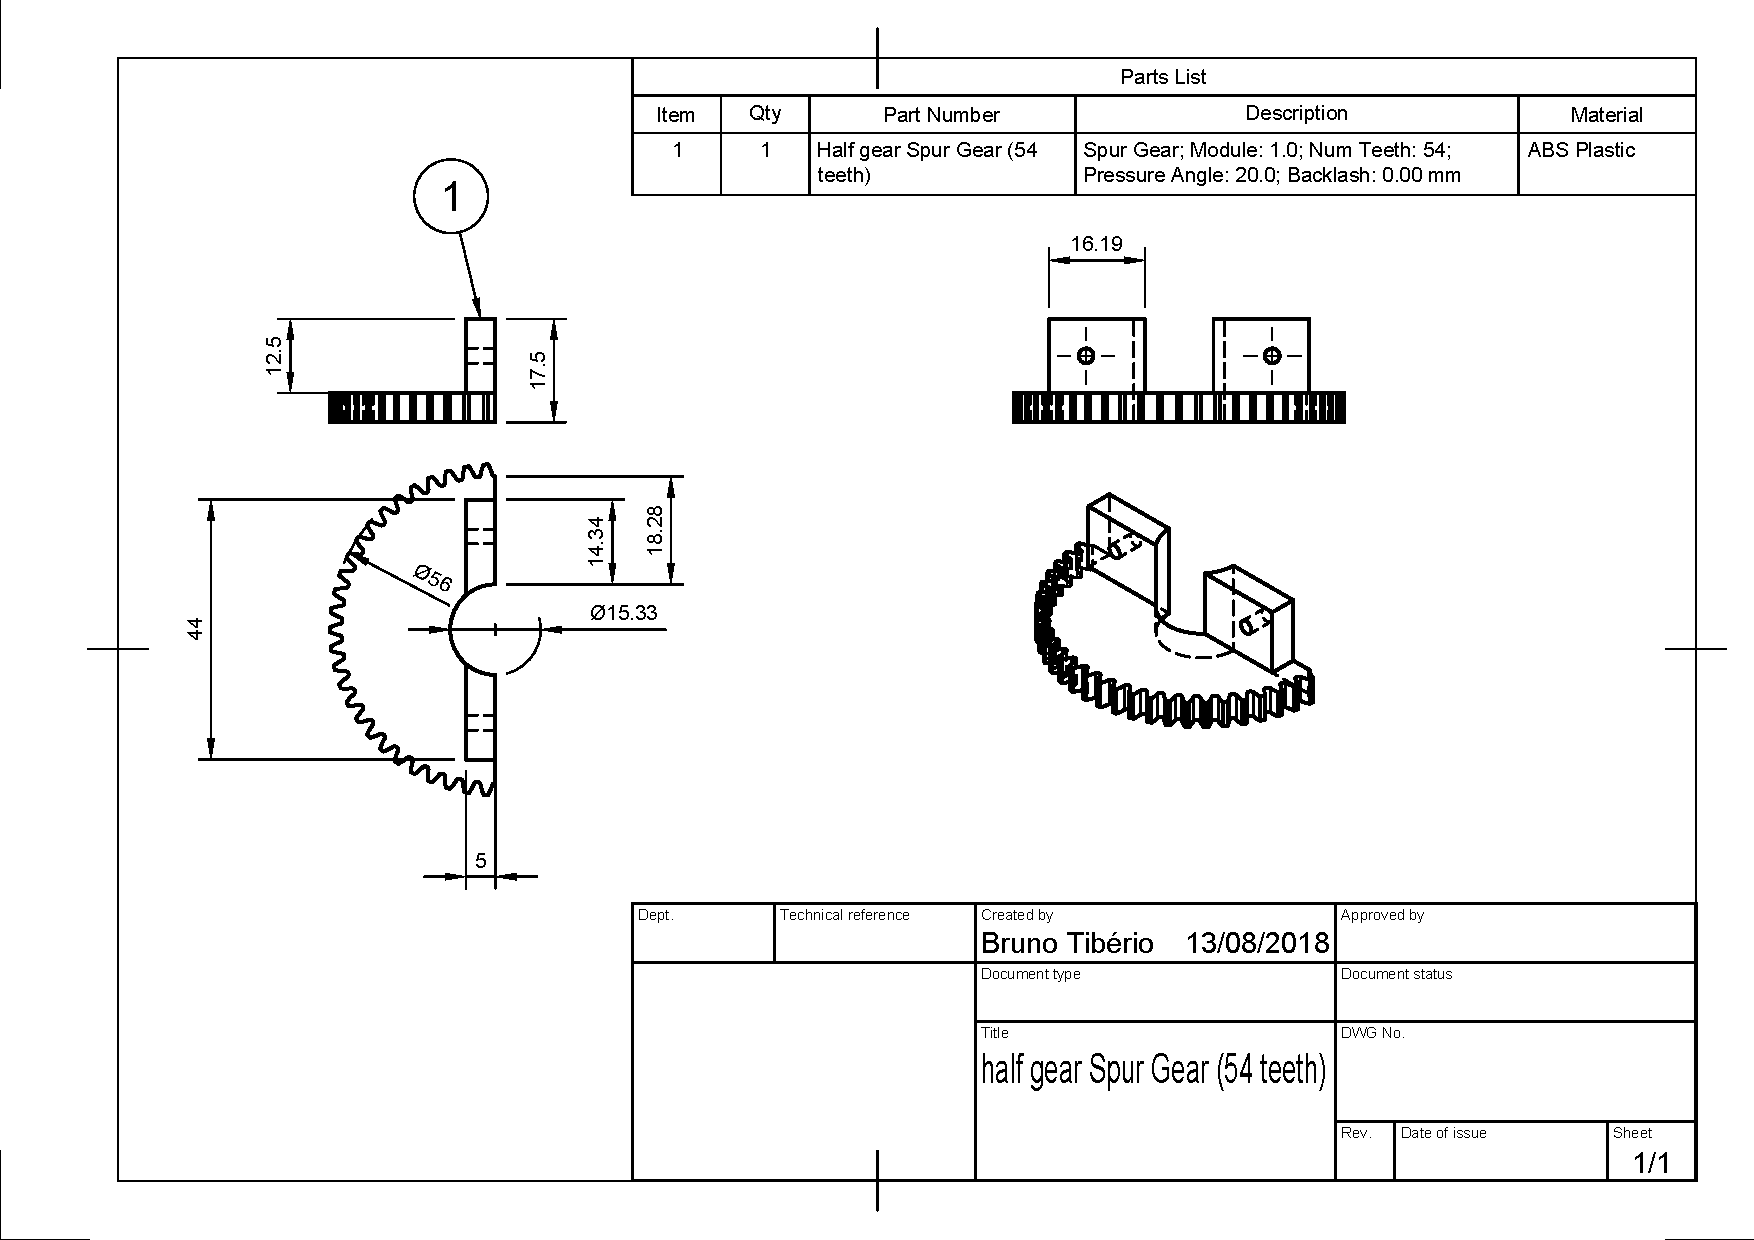
\includepdf[scale=0.8, landscape=true,pagecommand=\section{Half gear 54 teeth} \label{draw:half-gear}, trim=5mm 5mm 5mm 5mm,clip]{Drawings/half-gear}

%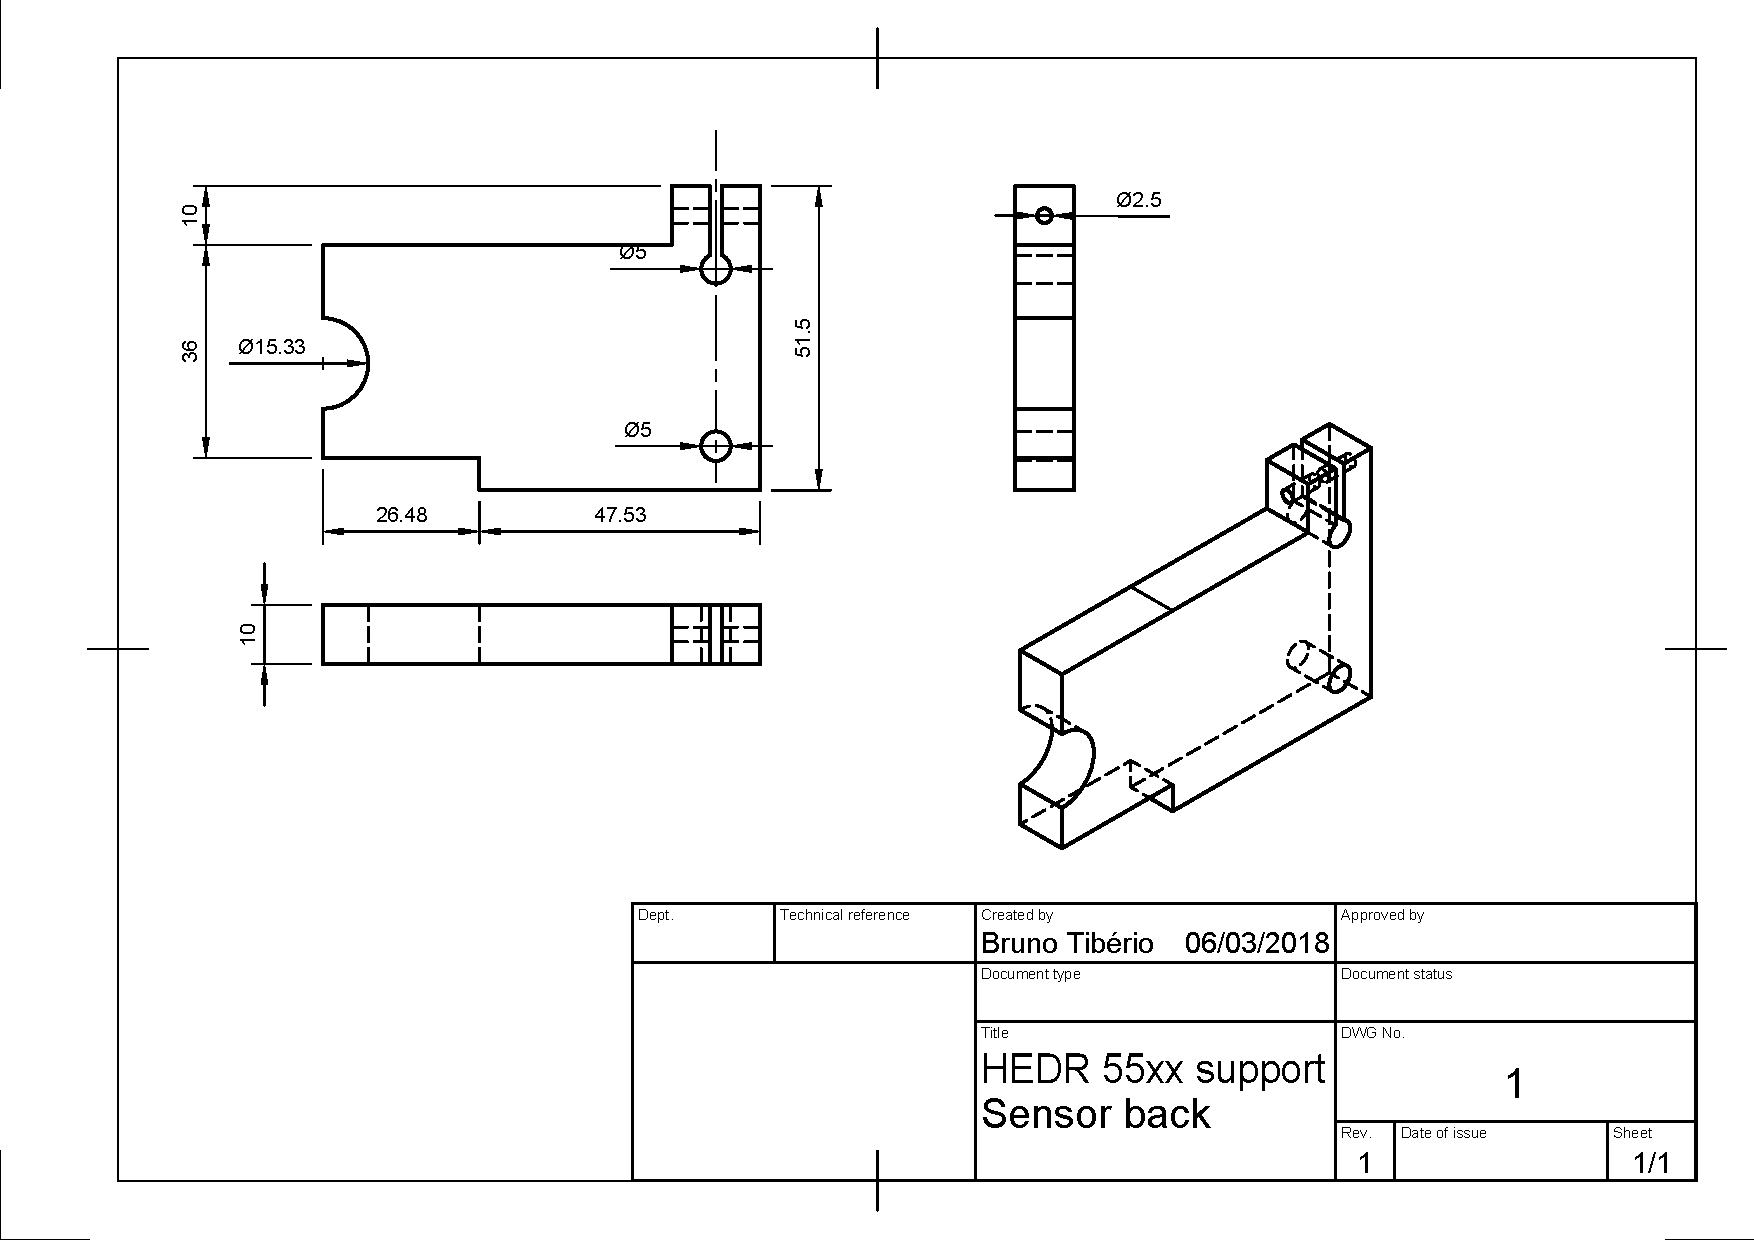
\includepdf[scale=0.75, angle=-90,pagecommand=\section{Sensor back spacer} \label{draw:sensor-back}, offset=0 -0.5cm, trim=5mm 5mm 5mm 5mm,clip]{Drawings/sensor-back}
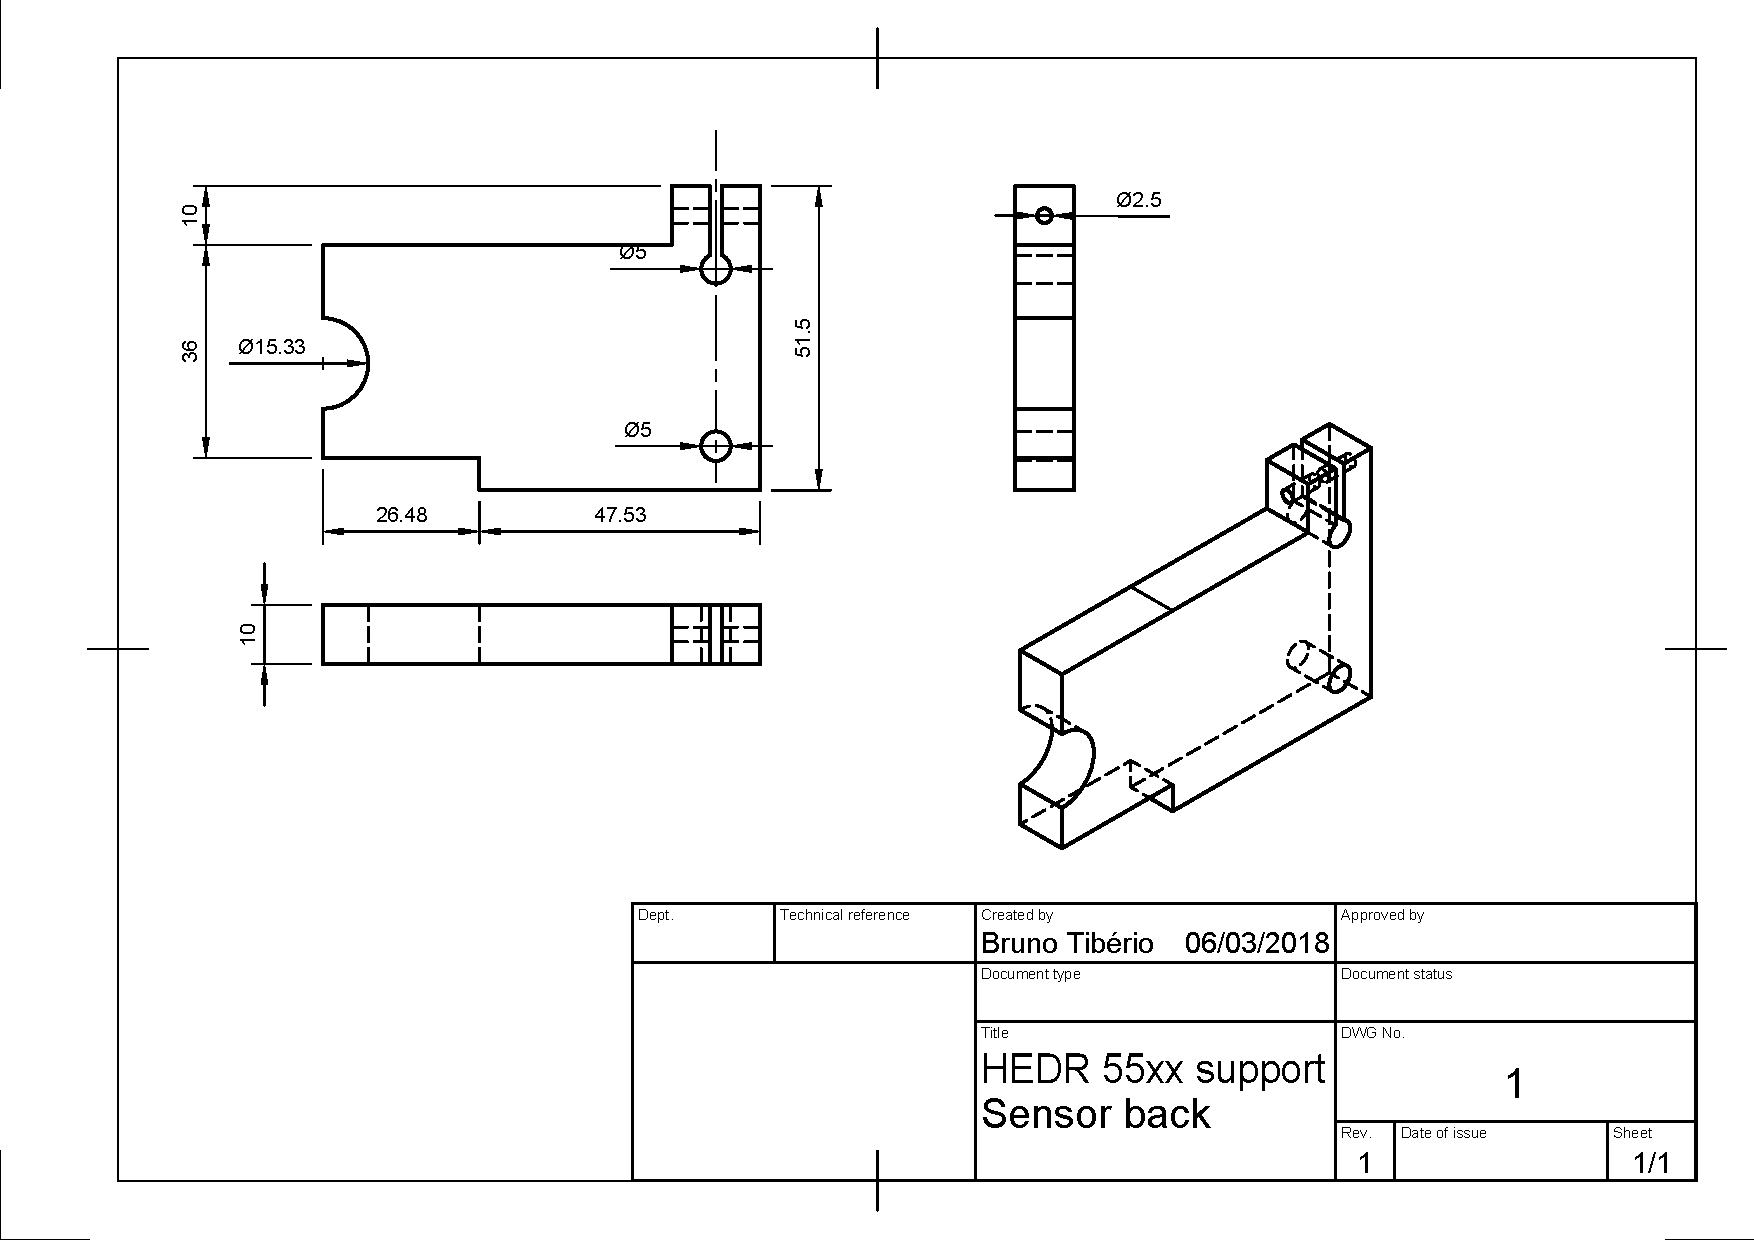
\includepdf[scale=0.8, landscape=true,pagecommand=\section{Sensor back spacer} \label{draw:sensor-back}, trim=5mm 5mm 5mm 5mm,clip]{Drawings/sensor-back}

%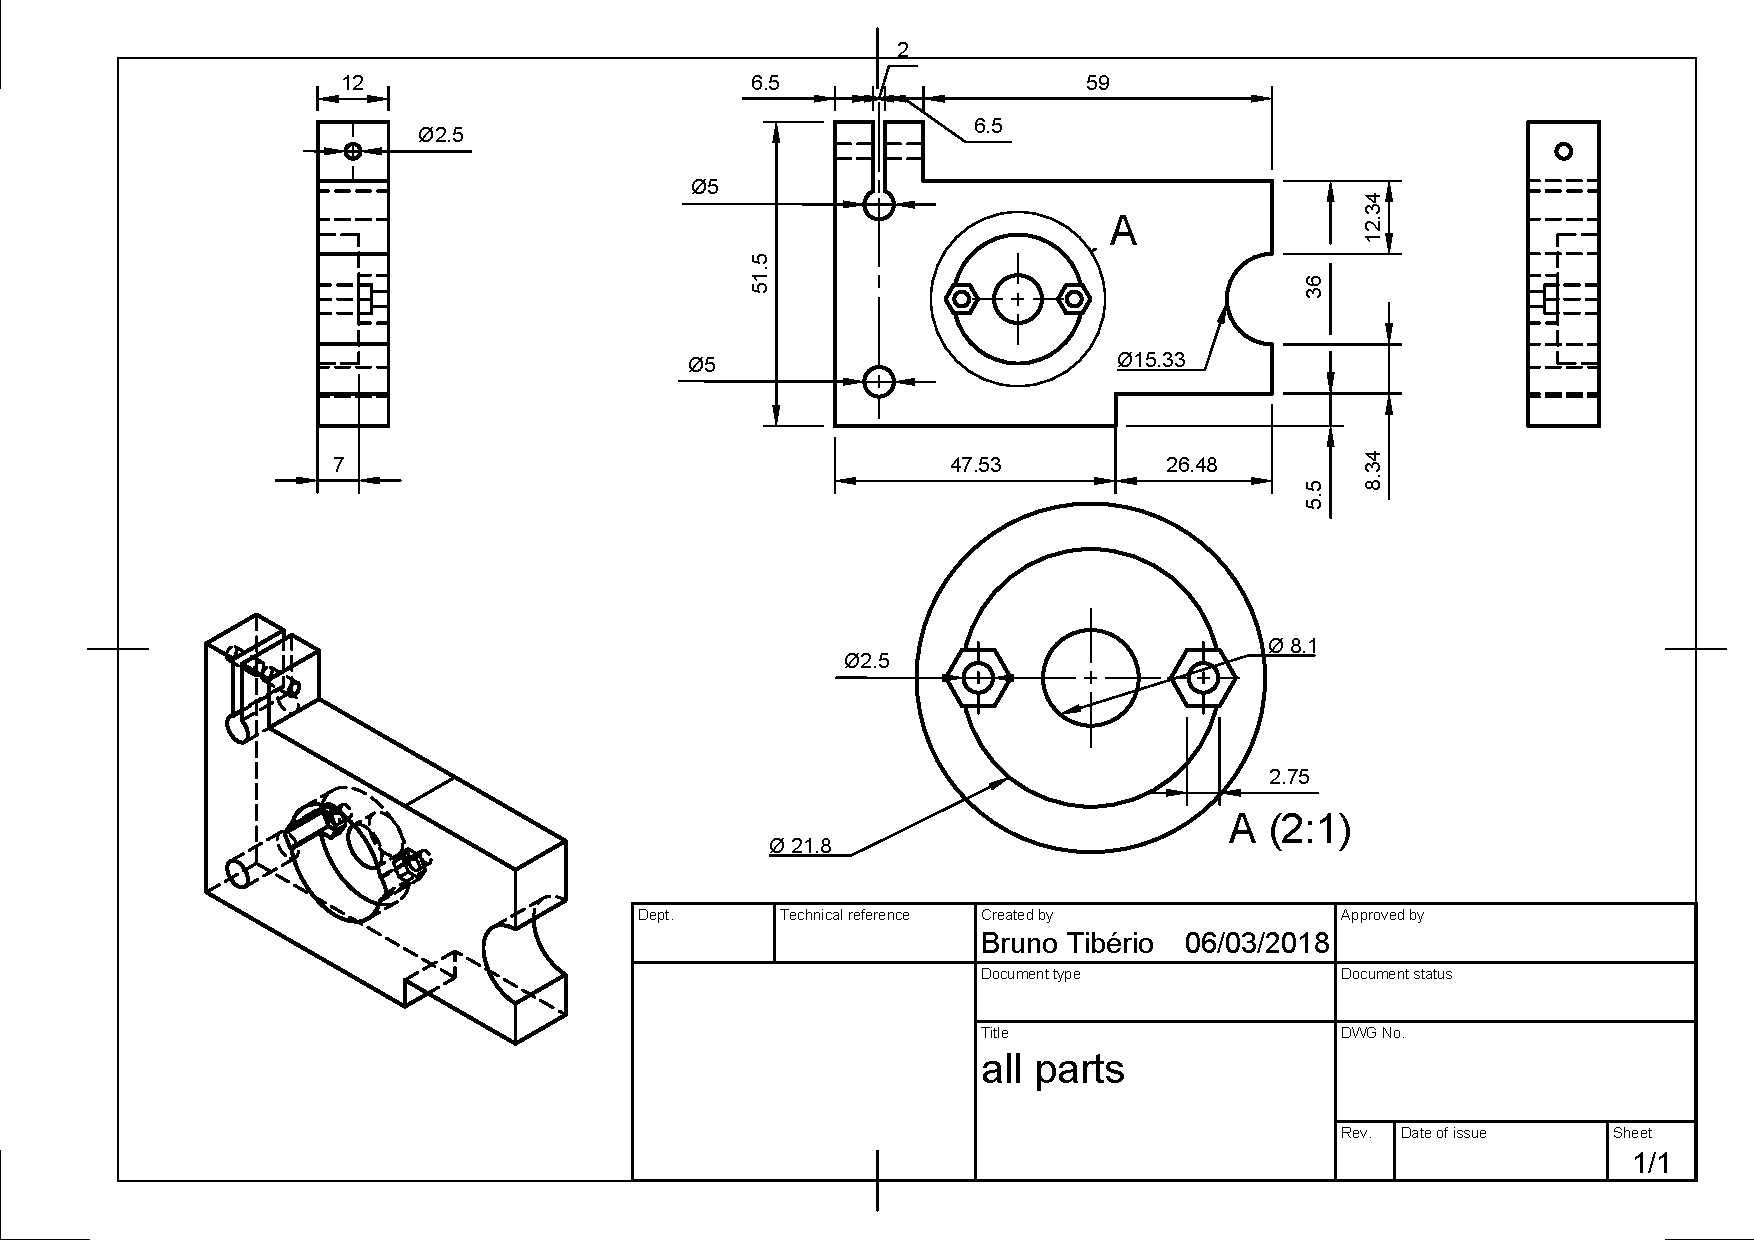
\includepdf[scale=0.75, angle=-90,pagecommand=\section{Sensor bearing holder} \label{draw:sensor-bearing-holder}, offset=0 -0.5cm, trim=5mm 5mm 5mm 5mm,clip]{Drawings/sensor-bearing-holder}
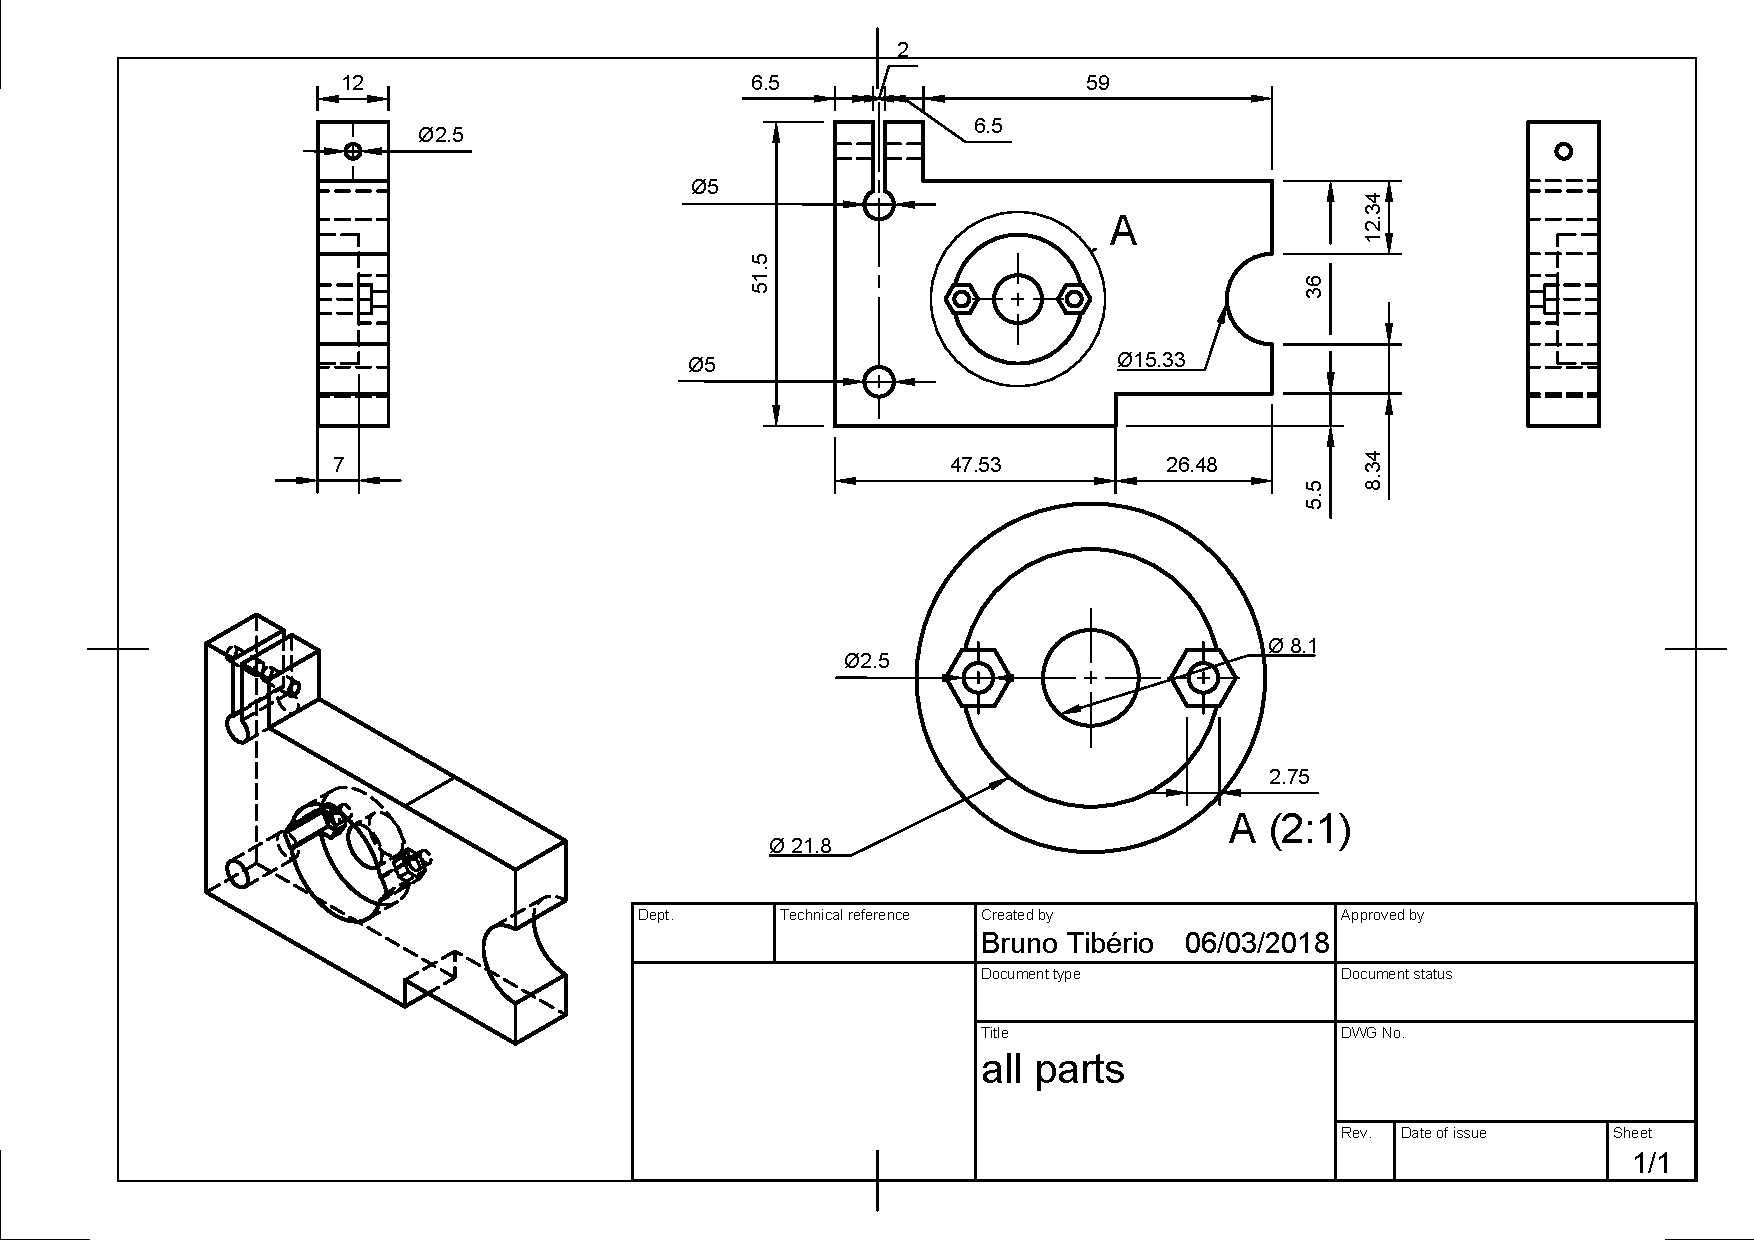
\includepdf[scale=0.8, landscape=true,pagecommand=\section{Sensor bearing holder} \label{draw:sensor-bearing-holder}, trim=5mm 5mm 5mm 5mm,clip]{Drawings/sensor-bearing-holder}


%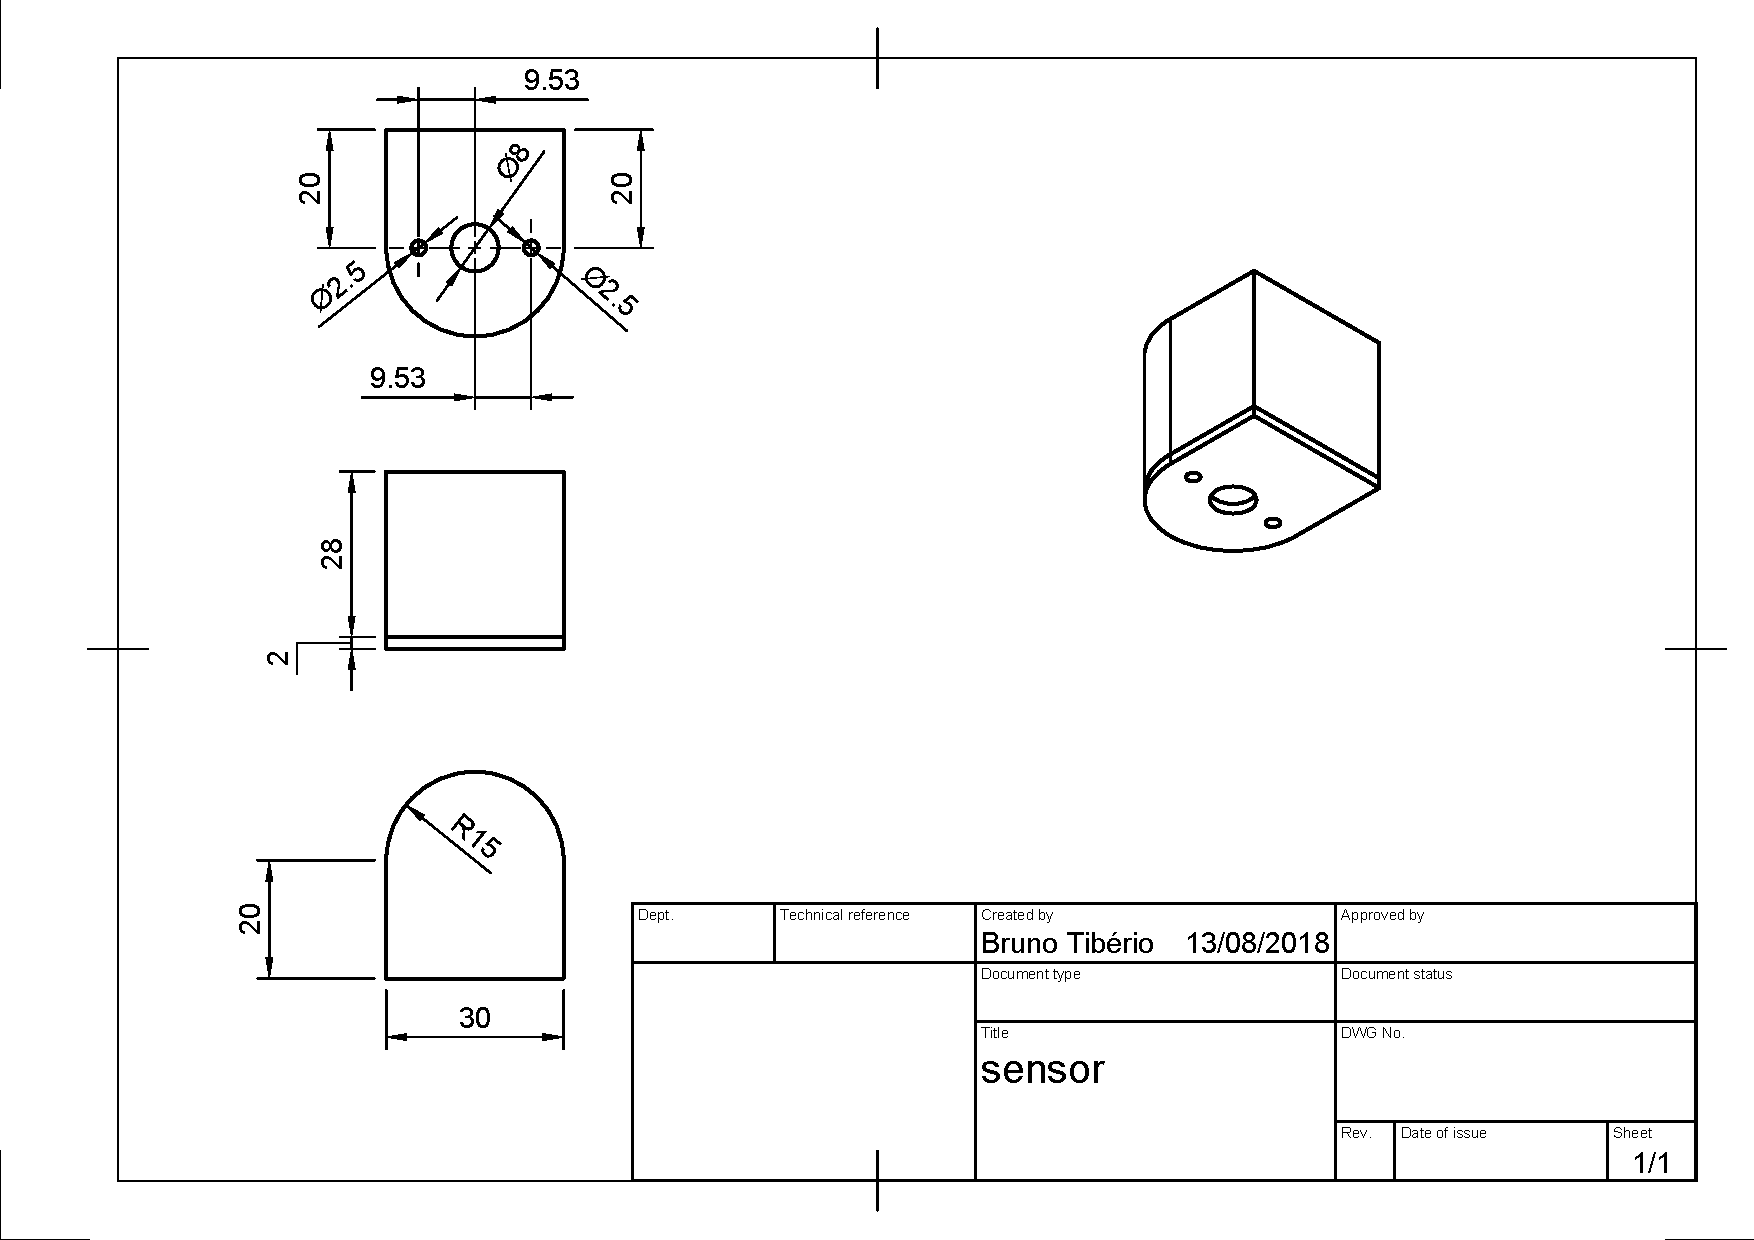
\includepdf[scale=0.75, angle=-90,pagecommand=\section{Sensor case} \label{draw:sensor-case}, offset=0 -0.5cm, trim=5mm 5mm 5mm 5mm,clip]{Drawings/sensor-case}
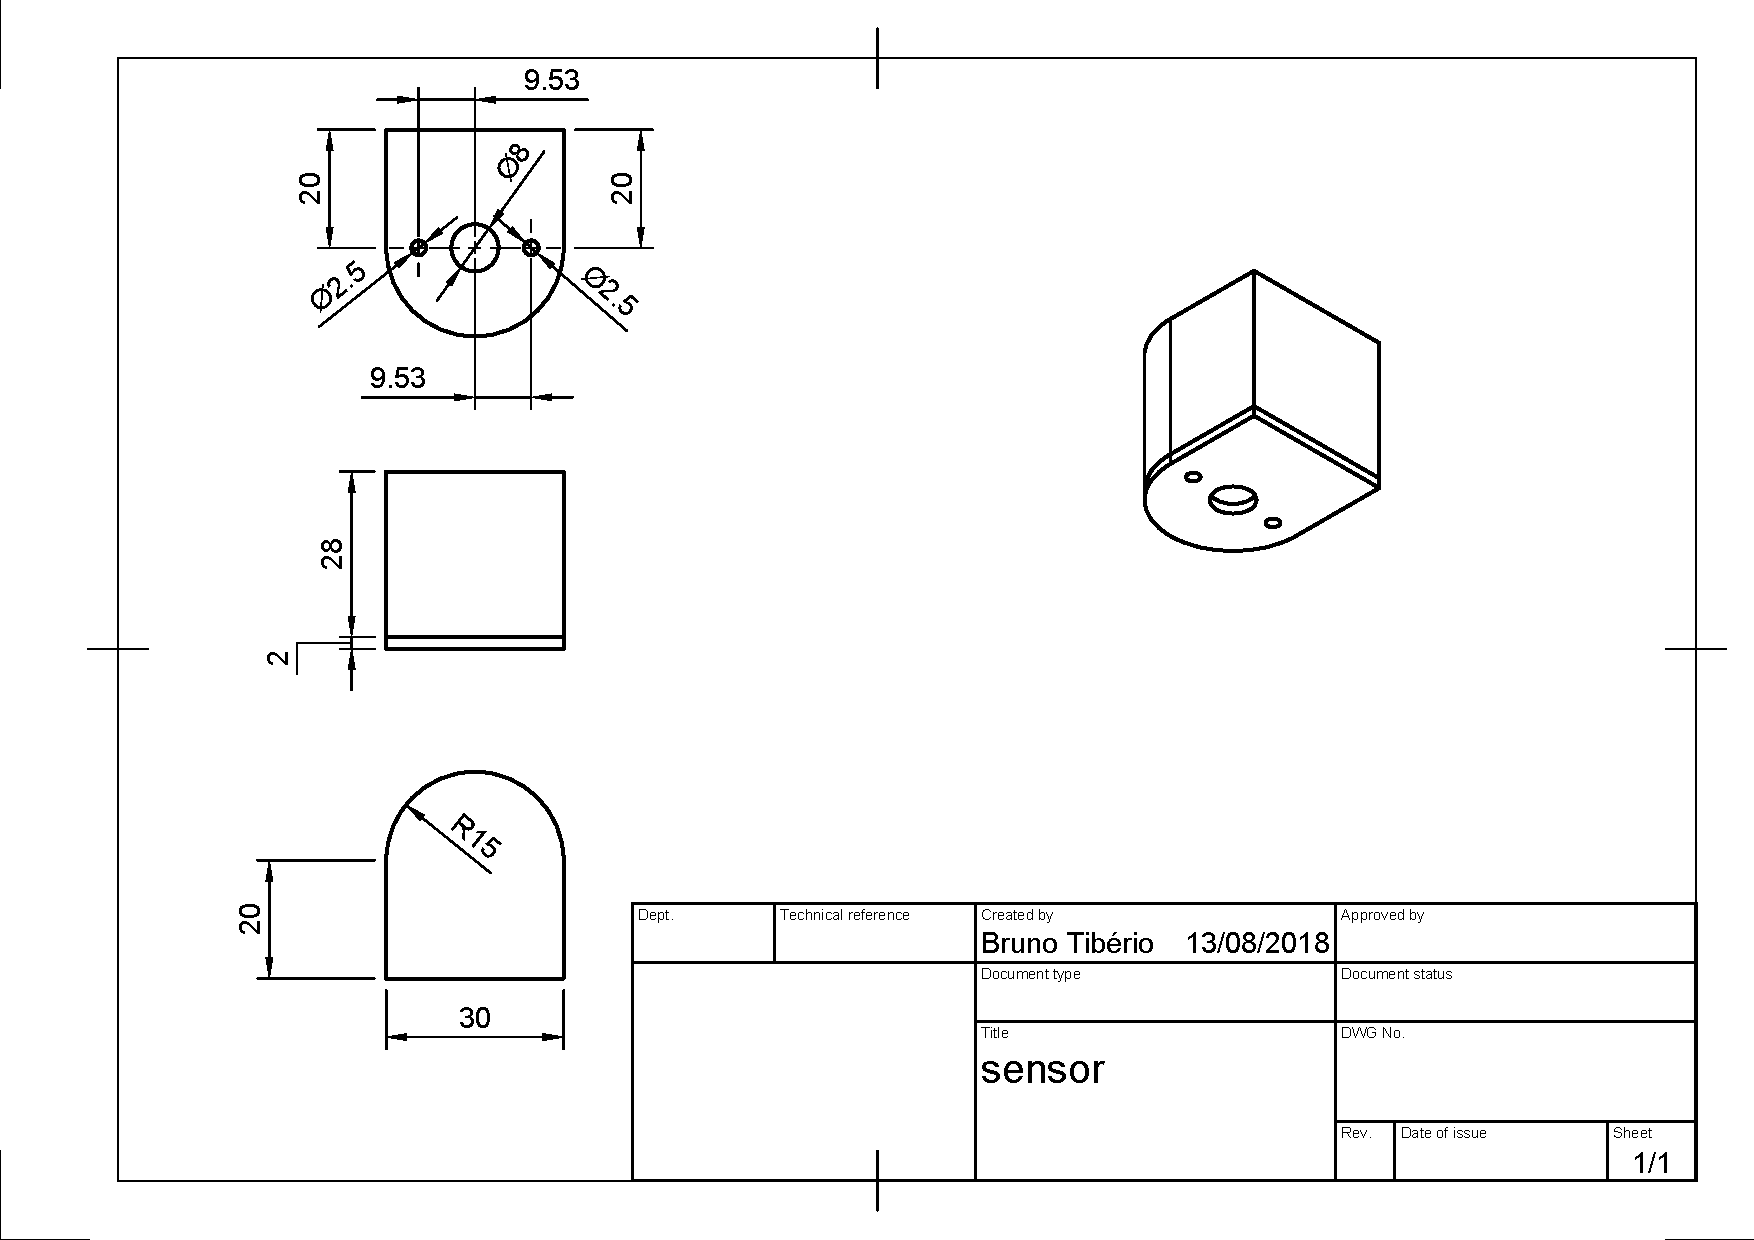
\includepdf[scale=0.8, landscape=true,pagecommand=\section{Sensor case} \label{draw:sensor-case}, trim=5mm 5mm 5mm 5mm,clip]{Drawings/sensor-case}

%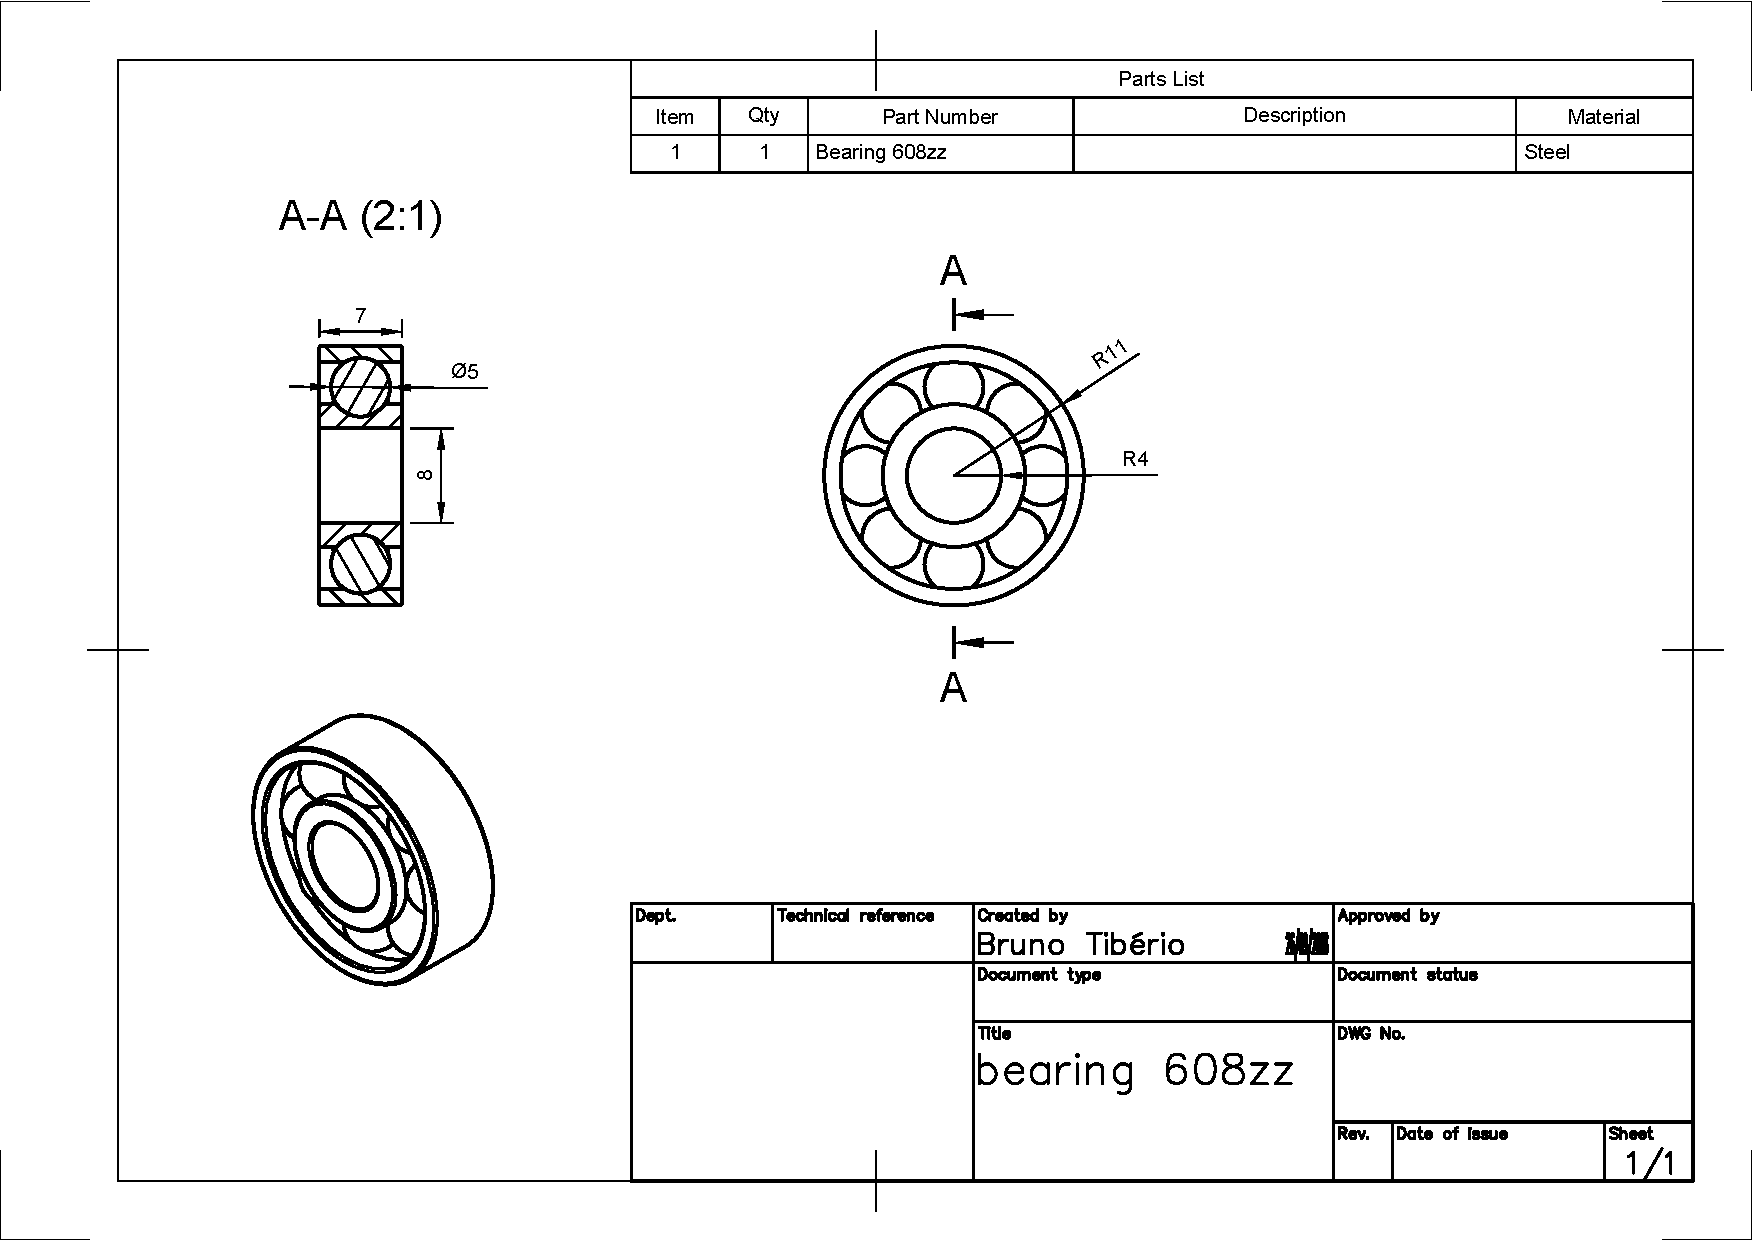
\includepdf[scale=0.75, angle=-90,pagecommand=\section{Bearing} \label{draw:bearing}, offset=0 -0.5cm, trim=5mm 5mm 5mm 5mm,clip]{Drawings/bearing-608zz}

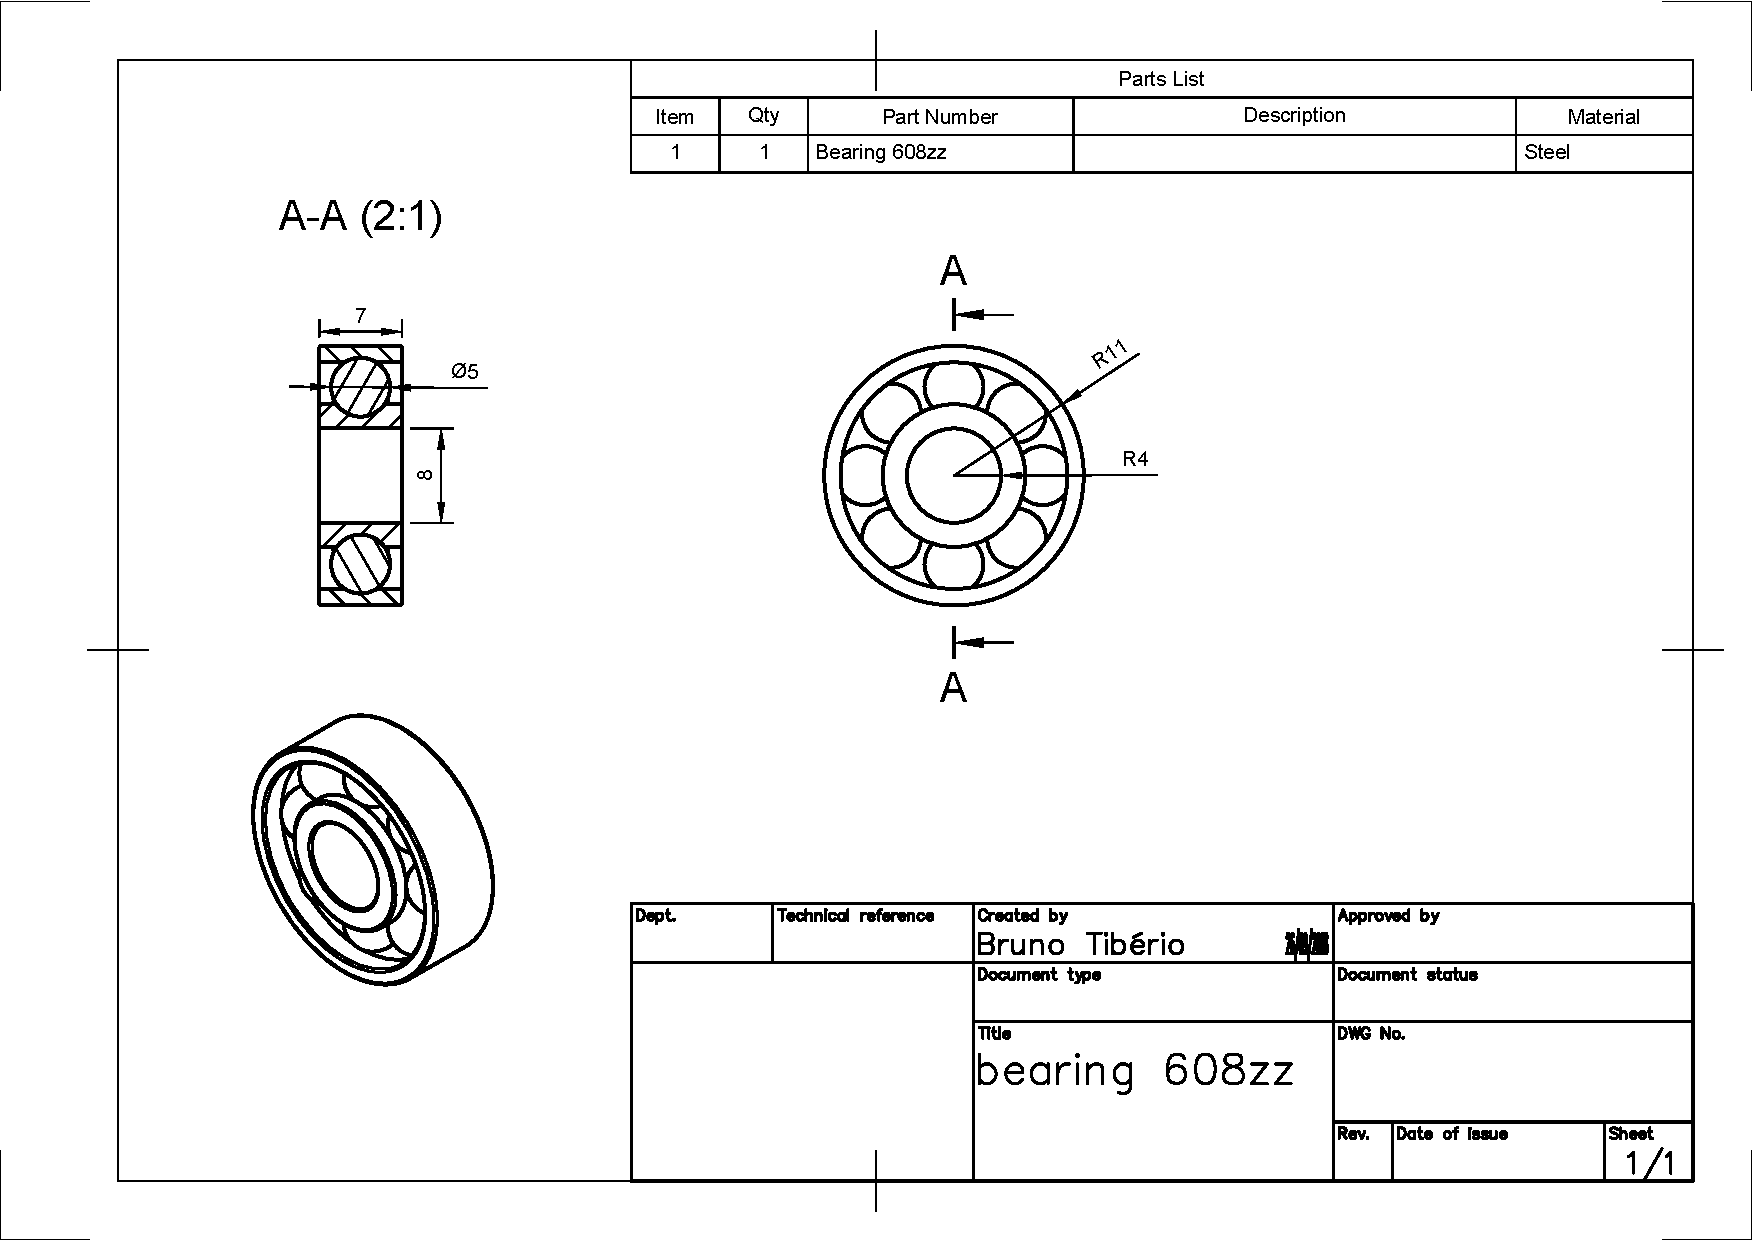
\includepdf[scale=0.8, landscape=true ,pagecommand=\section{Bearing} \label{draw:bearing},  trim=5mm 5mm 5mm 5mm,clip]{Drawings/bearing-608zz}

\cleardoublepage
\pagestyle{plain}

%------------------------------------------------------------------------
% add development board schematic as appendix
%------------------------------------------------------------------------
\setcounter{page}{1}
\pagestyle{plain}
\setlength{\voffset}{\originalVOffset}
\setlength{\hoffset}{\originalHOffset}
\chapter{Development CAN board schematics}
\label{appendix:can_schematics}
\vfill
\pagebreak
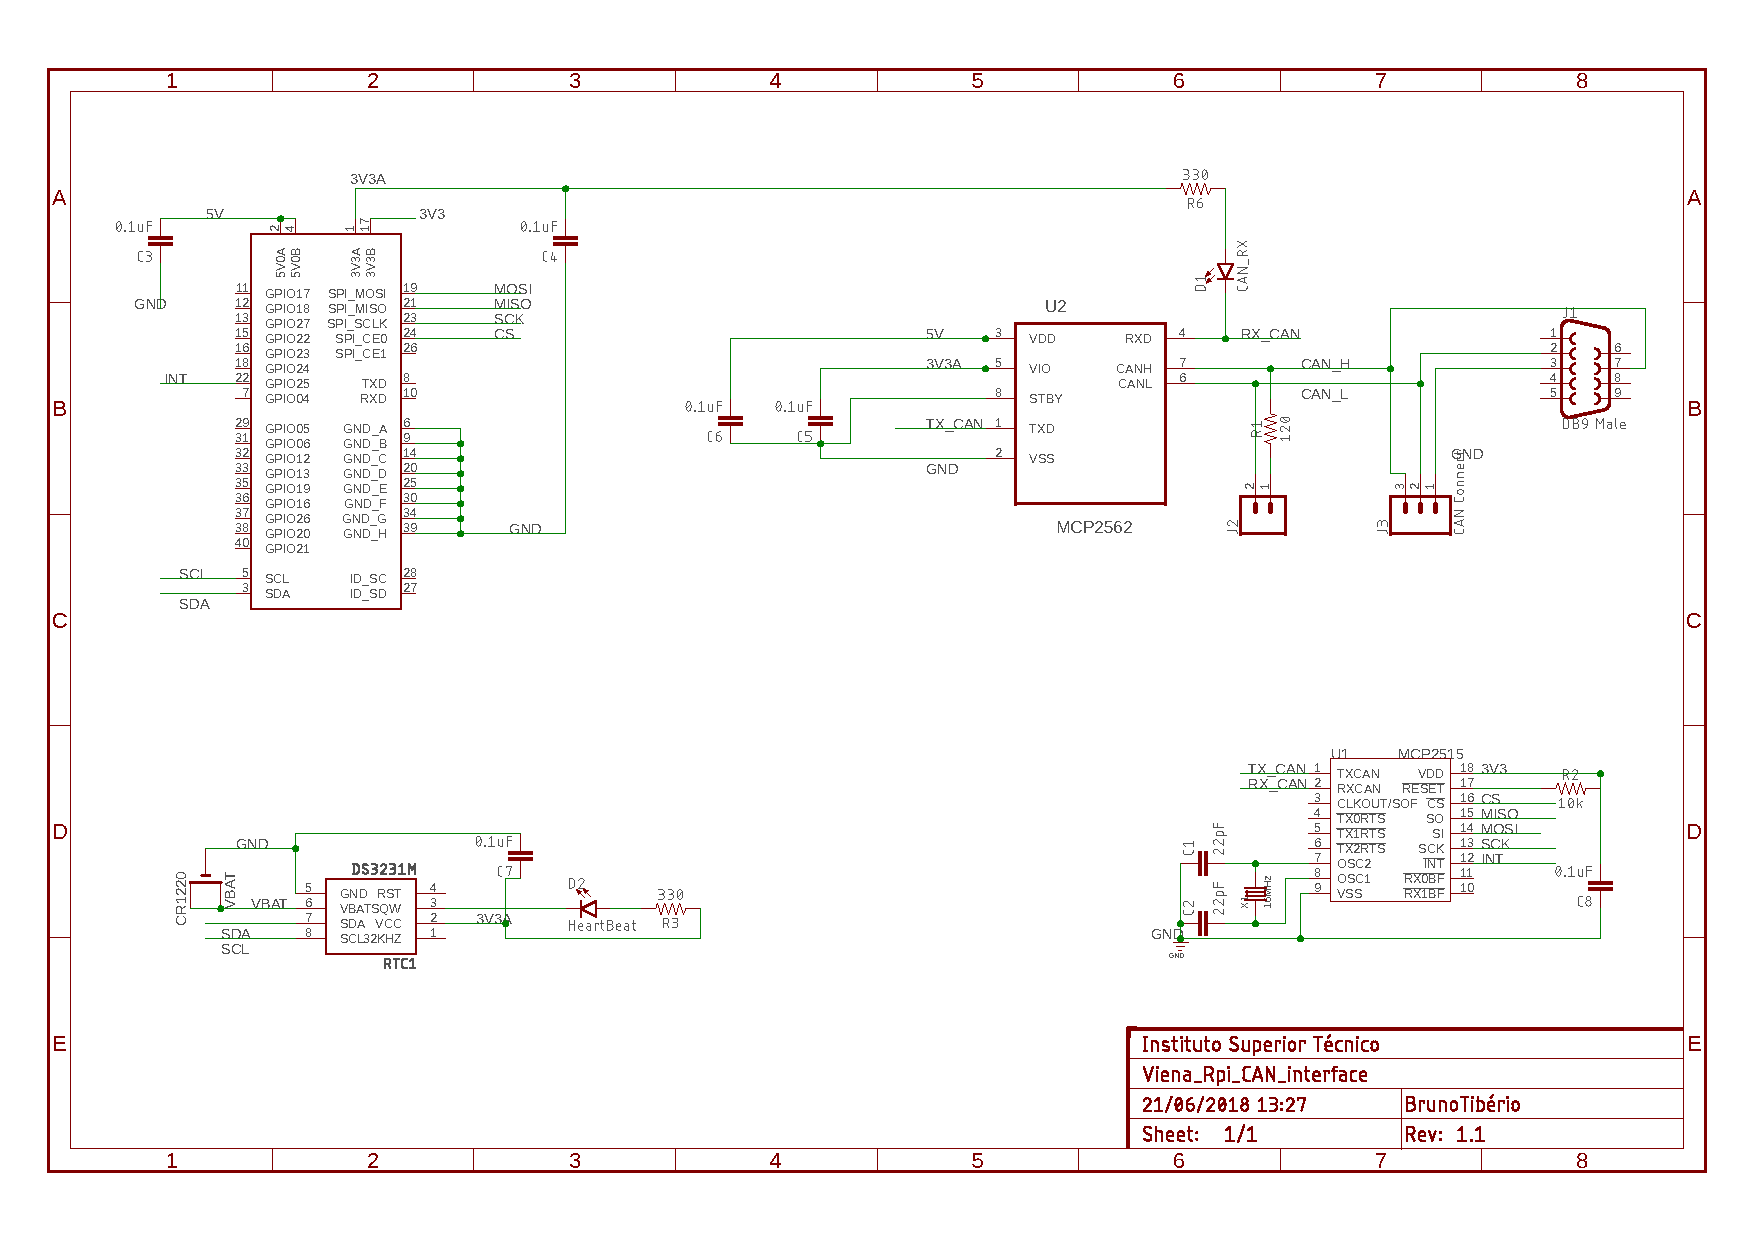
\includepdf[scale=0.9, landscape=true]{appendix/Viena_Rpi_CAN_interface.pdf}
\cleardoublepage

%------------------------------------------------------------------------
% add calibration script as appendix
%------------------------------------------------------------------------
\setcounter{page}{1}
\pagestyle{plain}
\chapter{Calibration script}
\label{appendix:calibration_script}
\lstinputlisting[language=Octave, 
				frame=None, 
				basicstyle=\small\ttfamily, 
				commentstyle=\color{greenmat},
				keywordstyle=\color{bluemat}]{appendix/find_calibration_parameters.m}
				
\cleardoublepage
%------------------------------------------------------------------------
% add steering class script as appendix
%------------------------------------------------------------------------
\setcounter{page}{1}
\pagestyle{empty}
\chapter{Steering controller}
\label{appendix:steering_script}
\cleardoublepage
\pagestyle{empty}
% cut header from pdf

\includepdf[pages=5, trim=0 0 0 5cm, clip, pagecommand=\section{Steering Controller - documentation}\label{appendix:steering_doc}]{appendix/SteeringControllerTester}

\includepdf[pages=6]{appendix/SteeringControllerTester}
\cleardoublepage
% add complete python code
%------------------------------------------------------------------------
% add calibration script as appendix
%------------------------------------------------------------------------
\setcounter{page}{1}
\pagestyle{plain}
\section{Steering Controller - script}
\label{appendix:steering_code}
\lstset{language=Python}
\lstinputlisting[language=python, 
frame=None, keywordstyle=\color{orange}, commentstyle=\color{greenmat}, basicstyle=\fontsize{7}{8}\ttfamily]{appendix/steering_controller.py}
\cleardoublepage

%------------------------------------------------------------------------
% add sinamics library doc as appendix
%------------------------------------------------------------------------
\setcounter{page}{1}
\pagestyle{empty}
\setlength{\voffset}{\originalVOffset}
\setlength{\hoffset}{\originalHOffset}
\chapter{Sinamics CANopen Library Documentation}
\cleardoublepage
\setlength{\voffset}{0cm}
\setlength{\hoffset}{0cm}
\label{appendix:sinamics}

\includepdf[pages=5-11]{appendix/sinamics-canopen}
\setlength{\voffset}{\originalVOffset}
\setlength{\hoffset}{\originalHOffset}
\cleardoublepage